%!TEX root = Projeto.tex
\subsection{Vulnerabilidades}
Violações de privacidade são possíveis nos navegadores por causa da natureza dinâmica da linguagem Javascript e de sua ausência de restrições de segurança em tempo de execução \cite{Jang2010}. Seus usuários estão expostos a ataques sutis com objetivos diversos como roubar \textit{cookies} e \textit{tokens} de autorização, redirecionar o navegador para sites falsos (\textit{phishing}), observar o histórico de navegação e rastrear o comportamento do usuário através dos movimentos do ponteiro do mouse e eventos de teclado. Para que {\scripts} mal-intencionados sejam incorporados a páginas benignas, \textit{hackers} fazem uso de vulnerabilidades como \textit{cross-site scripting (XSS)} \cite{OWASP:XSS} e comprometimento de extensões \cite{Heule2015_Most_Dangerous_Code} do navegador.

% \begin{todo}
% Aqui é preciso apresentar como este problema é caracterizado, nas referências cabíveis. Tudo indica que se trata de um "DOM-based XSS", que eu livremente traduzo como "XSS baseado em DOM" (péssimo). Imagino colocar a definição do OWASP e indicar as classificações do CWE (Common Weaknesses Enumeration) que orbitam em torno do problema.
% \end{todo}

\cite{OWASP:DOMXSS} define um ataque denominado ``XSS baseado em DOM'' como a modificação deliberada do modelo de objetos do navegador com o objetivo de influenciar seu ambiente de execução, sem que a visualização da página seja prejudicada ou que o navegador se comporte inesperadamente. Por essa característica, o usuário não percebe que pode haver um ataque em andamento.

\subsubsection{Mecanismos para propagação de informação suportados pelo navegador}
\label{Secao: Vulnerabilidades_MecanismosPropagacao}
\citeinline{Bielova2013} enumera os mecanismos que o navegador oferece para permitir comunicação entre uma aplicação web e outros recursos receptores de dados. A mera possibilidade de comunicação não constitui uma ameaça às aplicações, sendo de fato o meio de se viabilizar as principais funcionalidades do navegador. No entanto, autores de \scripts{} mal intencionados podem tirar proveito dos mecanismos de comunicação para propagar informação sensível.

\paragraph{APIs relevantes} % (fold)
\label{par:apis_relevantes}

\begin{description}
	\item[Objetos do DOM \poe{Core}] Toda a árvore de elementos HTML representada na estrutura do DOM, encabeçada pelo objeto |window.document|, corresponde à API \poe{core} do DOM. Todos os \scripts{} executando em um determinado domínio têm acesso ao mesmo objeto |document|. Não havendo garantias sobre as intenções de cada \script{} incorporado, cabe ao autor de uma aplicação web confiar que o comportamento desses \scripts{} não é malicioso do ponto de vista da segurança da informação.
	\item[Domínio] O domínio associado a uma aplicação web é refletido pela propriedade do DOM |document.domain|, que pode ser modificada por \scripts{}. Um exemplo dessa operação é proporcionado por dois \scripts{}, um executando em um domínio \location{a.app.com} e outro no domínio \location{b.app.com}. Ambos podem alterar seus domínios de origem para \location{app.com}, o que os fará compartilharem o mesmo DOM. Por meio dessa operação os \scripts{} ``relaxam'' a amplitude do domínio relevante para as restrições derivadas da SOP.
\end{description}

% paragraph apis_relevantes (end)


\subsubsection{Compartilhamento do ambiente de execução}
Tanto o código \poe{inline} quanto os {\scripts} baixados pelas páginas da web são executados com os mesmos privilégios e mesmo nível de acesso à estrutura de documento do navegador \cite[p. 2-3]{DeRyck2012}, não importando o domínio de origem dos {\scripts}. A esse respeito, \citeinline{Nikiforakis2012}, em sua \poe{survey} a respeito da inclusão de código Javascript hospedado em múltiplas origens, descreve esta forma de incorporação de {\scripts} como uma expansão do ``perímetro de segurança'' da página, atribuindo a terceiros o mesmo nível de confiança dado aos {\scripts} desenvolvidos pelos autores diretos de uma aplicação web.

{\Scripts} mantidos por terceiros podem sofrer modificações não previstas pelas aplicações que os hospedam, o que tem o potencial de introduzir \poe{bugs} ou comportamento inadequado ou hostil. Uma demonstração do problema pode ser exemplificada na figura \ref{Fig: diagrama01} e listagem de código \ref{Src: webPageMultiOrigin}. Nesse exemplo, um {\script} tido como benigno é incorporado a uma página web a partir de um domínio de CDN (\poe{content delivery network}), diferente daquele da aplicação que efetivamente publica a página. O servidor desse {\script}, pelo protocolo CORS, sinaliza ao navegador que o domínio da página é confiável. O {\script} externo pode, então, iniciar requisições ao seu domínio de origem -- uma consequência desejada pelos autores da página, pois o {\script} depende desse acesso para efetuar suas funções.

\begin{figure}
	\centering
	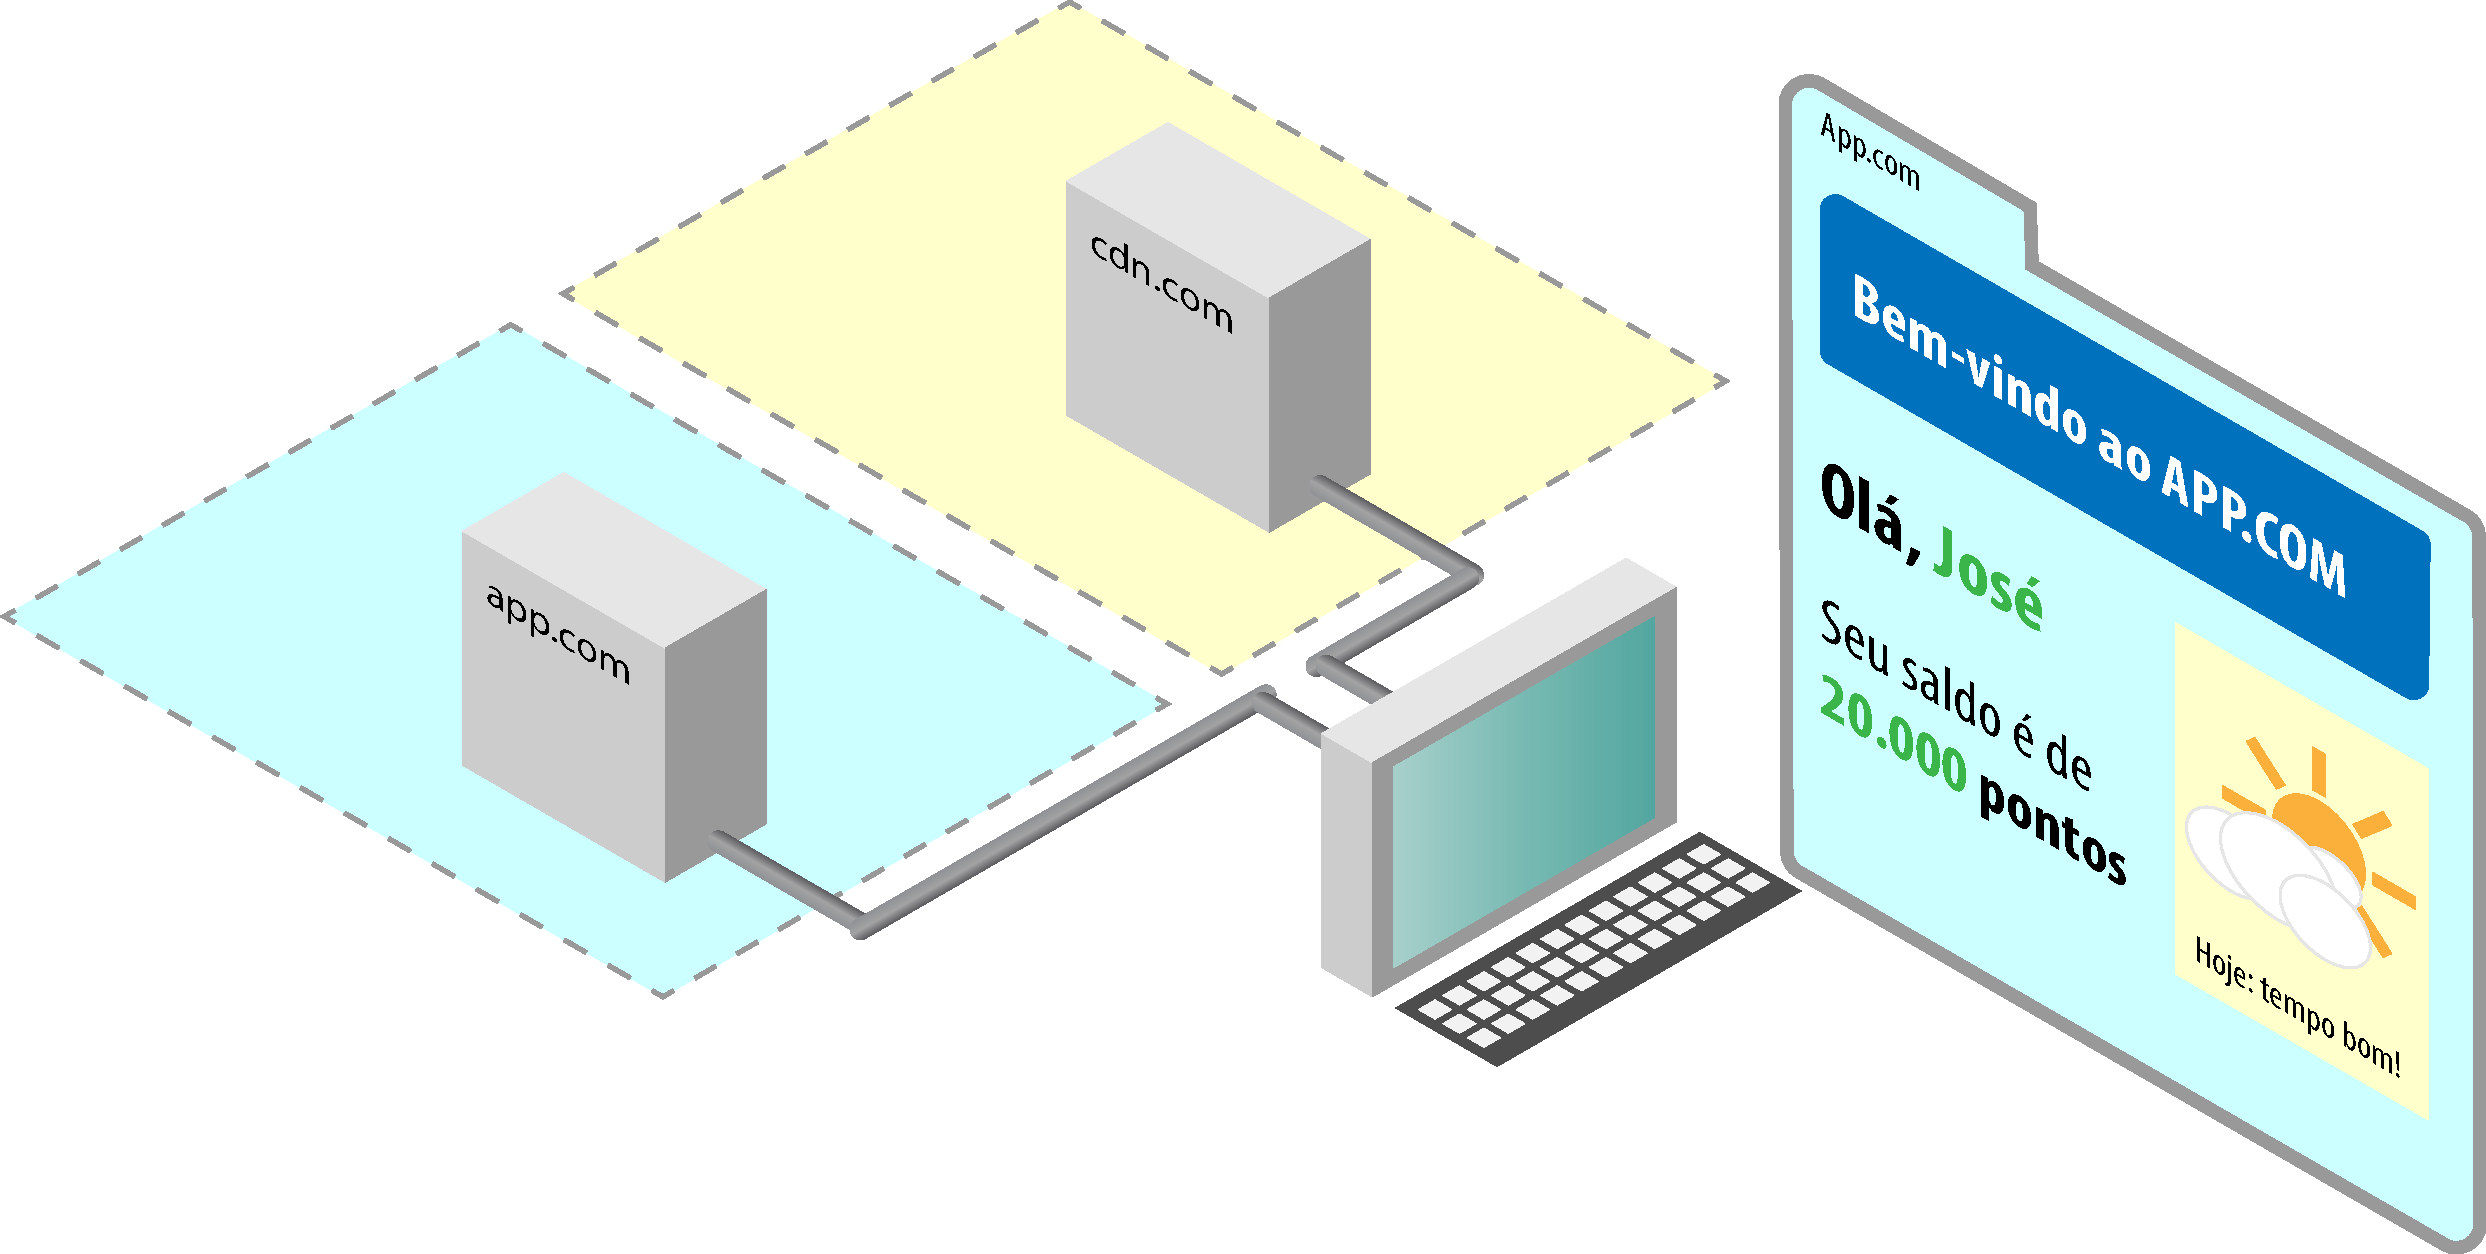
\includegraphics[width=10cm]{diagramas/diagrama01.pdf}
	\caption{Aplicação web composta por conteúdo proveniente de duas origens.}
	\label{Fig: diagrama01}
	
	\lstinputlisting[language=html,
	inputencoding=utf8,
	label={Src: webPageMultiOrigin},
	caption={[Página HTML incorporando {\script} de outra origem]Incorporação de {\script} de outra origem (linha \ref{lstCdnScript})}]{codigo/sample01-leaking-script.html}
\end{figure}

Em momento posterior, o {\script} servido pelos servidores da CDN é substituído por código malicioso que, além de efetuar as funções do {\script} benigno, captura o conteúdo da página armazenado no DOM (figura \ref{Fig: diagrama02}). O {\script} pode buscar informações específicas e potencialmente sensíveis como identificação do usuário, senhas e endereços. Por causa da autorização concedida pelo protocolo CORS, o código mal intencionado tem a chance de transmitir o conteúdo capturado para um serviço anômalo hospedado no mesmo domínio do {\script}.

\begin{figure}
	\centering
	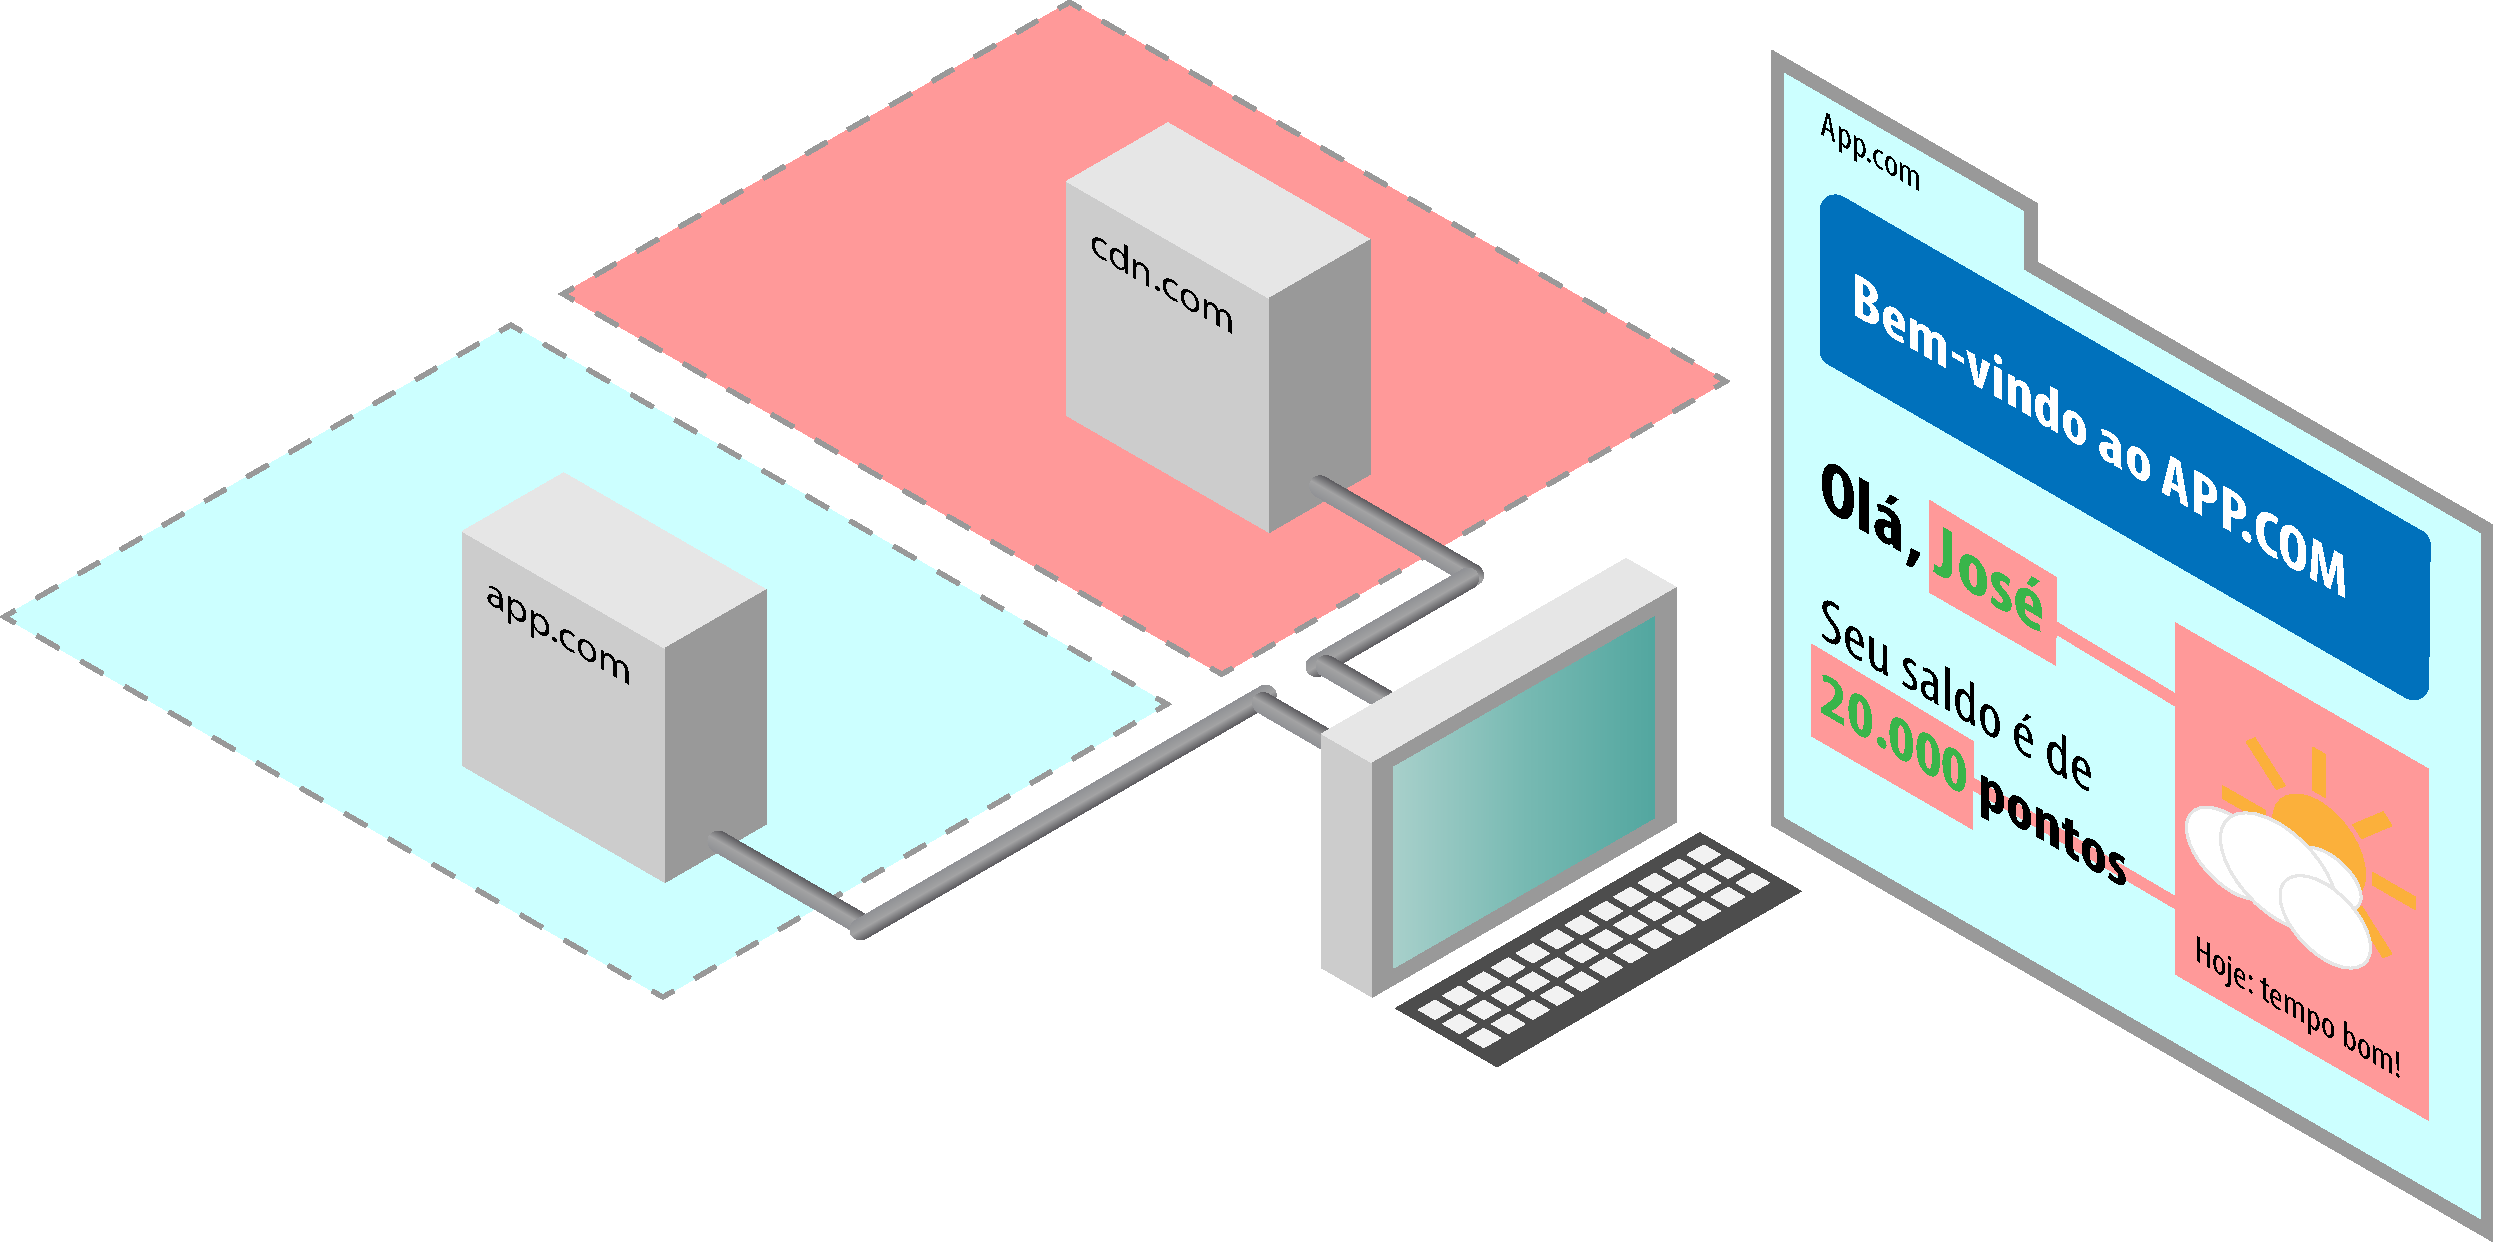
\includegraphics[width=10cm]{diagramas/diagrama02.pdf}
	\caption{Domínio de CDN comprometido, capturando informações do usuário.}
	\label{Fig: diagrama02}
\end{figure}

Acessar, capturar e modificar informações contidas no DOM também são efeitos de extensões do navegador. Mas, diferentemente dos {\scripts} incorporados em páginas, extensões são executadas em modo privilegiado e podem afetar todas as páginas carregadas pelo navegador, não sendo confinadas a domínios específicos. Extensões como as do Google Chrome são publicadas exclusivamente em site específico e protegido, mas não é impossível que o código fonte de extensões seja descaracterizado e publicado pela ação de \poe{hackers} \cite{Spring2017}, afetando a todos os usuários que atualizarem a extensão -- um processo automático por padrão \cite{Google2017}.


\subsubsection{Cross-Site Scripting (XSS)}
Em Javascript, todos os recursos de código carregados dentro de uma mesma página possuem os mesmos privilégios de execução. Ataques do tipo \poe{cross-site scripting} tiram proveito dessa característica para injetar código malicioso em contextos onde seja possível observar e retransmitir informação sigilosa como \poe{cookies} do usuário, endereço do navegador, conteúdo de formulários, ou qualquer outra informação mantida pelo DOM.

O emprego de medidas para prevenção de ataques XSS \cite{OWASP:XSS-CheatSheet} \dubious{(QUAIS?)} não elimina riscos inerentes à tecnologia do navegador. Uma vez que componentes incorporados, como anúncios e \poe{players} de mídia, conseguem carregar {\scripts} tidos como confiáveis dinamicamente, um único trecho de código comprometido pode colocar informações em risco sem qualquer interferência dos dispositivos de segurança.

%\subsubsection{Sobrescrita do DOM} DOM CLOBBERING

%\subsubsection{Scraping} OWASP OAT-011

\subsubsection{Comprometimento de extensões}
Os mecanismos de extensibilidade oferecidos pelos navegadores melhoram a funcionalidade da web para os usuários, e o código de que são feitos é executado com privilégios mais elevados do que o dos {\scripts} incorporados pelos \poe{sites}. Por isso, os usuários precisam confirmar ao navegador que aceitam que uma extensão seja instalada, sendo informados a respeito dos privilégios que a extensão pretende utilizar. O fato de que esse processo precise se repetir a cada vez que uma extensão requisitar de um conjunto de privilégios diferente faz com que os desenvolvedores optem por solicitar, de antemão, uma gama de privilégios maior que a estritamente necessária \cite{Heule2015_Most_Dangerous_Code}.

Uma extensão que tiver sido comprometida (por exemplo, ao usar {\scripts} de terceiros que, por sua vez, tenham sido redirecionados ou adulterados) terá assim poder para ler e transmitir todo o conteúdo carregado e exibido pelo navegador, com o potencial de causar os mesmos efeitos observados em um ataque XSS, mas em escopo e poder aumentados, já que poderiam afetar todas as páginas abertas e todas as APIs publicadas pelo navegador.

%\tbc